%!TEX TS-program = pdflatex
%!TEX root = i3det-top.tex
%!TEX encoding = UTF-8 Unicode

\section{IceCube Online Systems}
\label{sec:online}
\textsl{(John K; 12-15 pages)}

%The division between \textit{triggering} and
%\textit{filtering} is the urgency of the processing.
%Triggers must operate within a bounded time and if not
%data is lost.  Filters operate behind such large buffers
%that this is not a consideration.  Historically this means
%that the triggers have been rather \emph{dumb} but there
%is in principle no ceiling to the trigger complexity.

\subsection{Data Flow Overview}

An overview of the data flow from DOMs to the satellite.  Description of
architecture and levels of data reduction, starting with a review of LC and
proceeding to triggers and then filters.  Secondary streams and SNDAQ.
I3Live, experiment control, and monitoring.

Figure: data flow diagram indicating major subsystems to be described in
this section: DAQ (incl. SNDAQ), PnF, I3Live, and SPADE/JADE.

\subsection{SPS and SPTS}

South Pole System: breakdown of computing hardware used at the pole between
hubs, DAQ, PnF, other machines, and infrastructure.  Internal network
bandwidth.  Redundancy, system monitoring (Nagios), and paging system.

Brief mention of SPTS as northern test and validation system.  Replay
capabilities.  

\subsection{Data Readout and Timing}
\subsubsection{Communications and Cable Bandwidth}

Description of communications protocol and messaging strategy.  Reference
to RAPCal and how it fits in.

% Q: is LC signaling documented anywhere yet?  Should it go here?

\subsubsection{Master Clock System}

The GPS clock and time string fanout tree, from master clock (and hot
spare), to Tier I and Tier II fanouts, the DSB card, and into the DOR card.

\subsubsection{DOR Card and Driver}

DOR card description: comms / readout, power control and measurement,
RAPCal initiation, and clock string readout.  Clock modes (internal /
external).  DOMs per card and cards per hub.

Brief description of driver.  Proc file interface.  Data transfer over PCI
bus via DMA.  

Figure: Combined clock fanout tree hierarchy and hub diagram (DSB and DOR
cards, power distribution).

\subsection{Processing at the Surface}
\textsl{(Dave G; 2-3 pages)}

Big-picture description of what DAQ does: collecting hits from the DOMs,
triggering on HLC hits, and packaging waveforms into events.  

\subsubsection{DOMHub and Hit Spooling}

Responsibility of StringHub.  Splicer and description of HKN1 algorithm.
Forwarding of HLC hit times to trigger.  Translation of DOR times into
UTC.  Servicing event readout requests (defer discussion to event builder
section).  Generation of secondary streams. 

Hitspooling.  Mention of hit daemon plans.  

\subsubsection{Supernova System}

SN secondary stream from DOMs and SNDAQ reference.  Interface to
hitspooling.  

\begin{figure}
 \begin{minipage}[t]{0.45\linewidth}
 \centering
  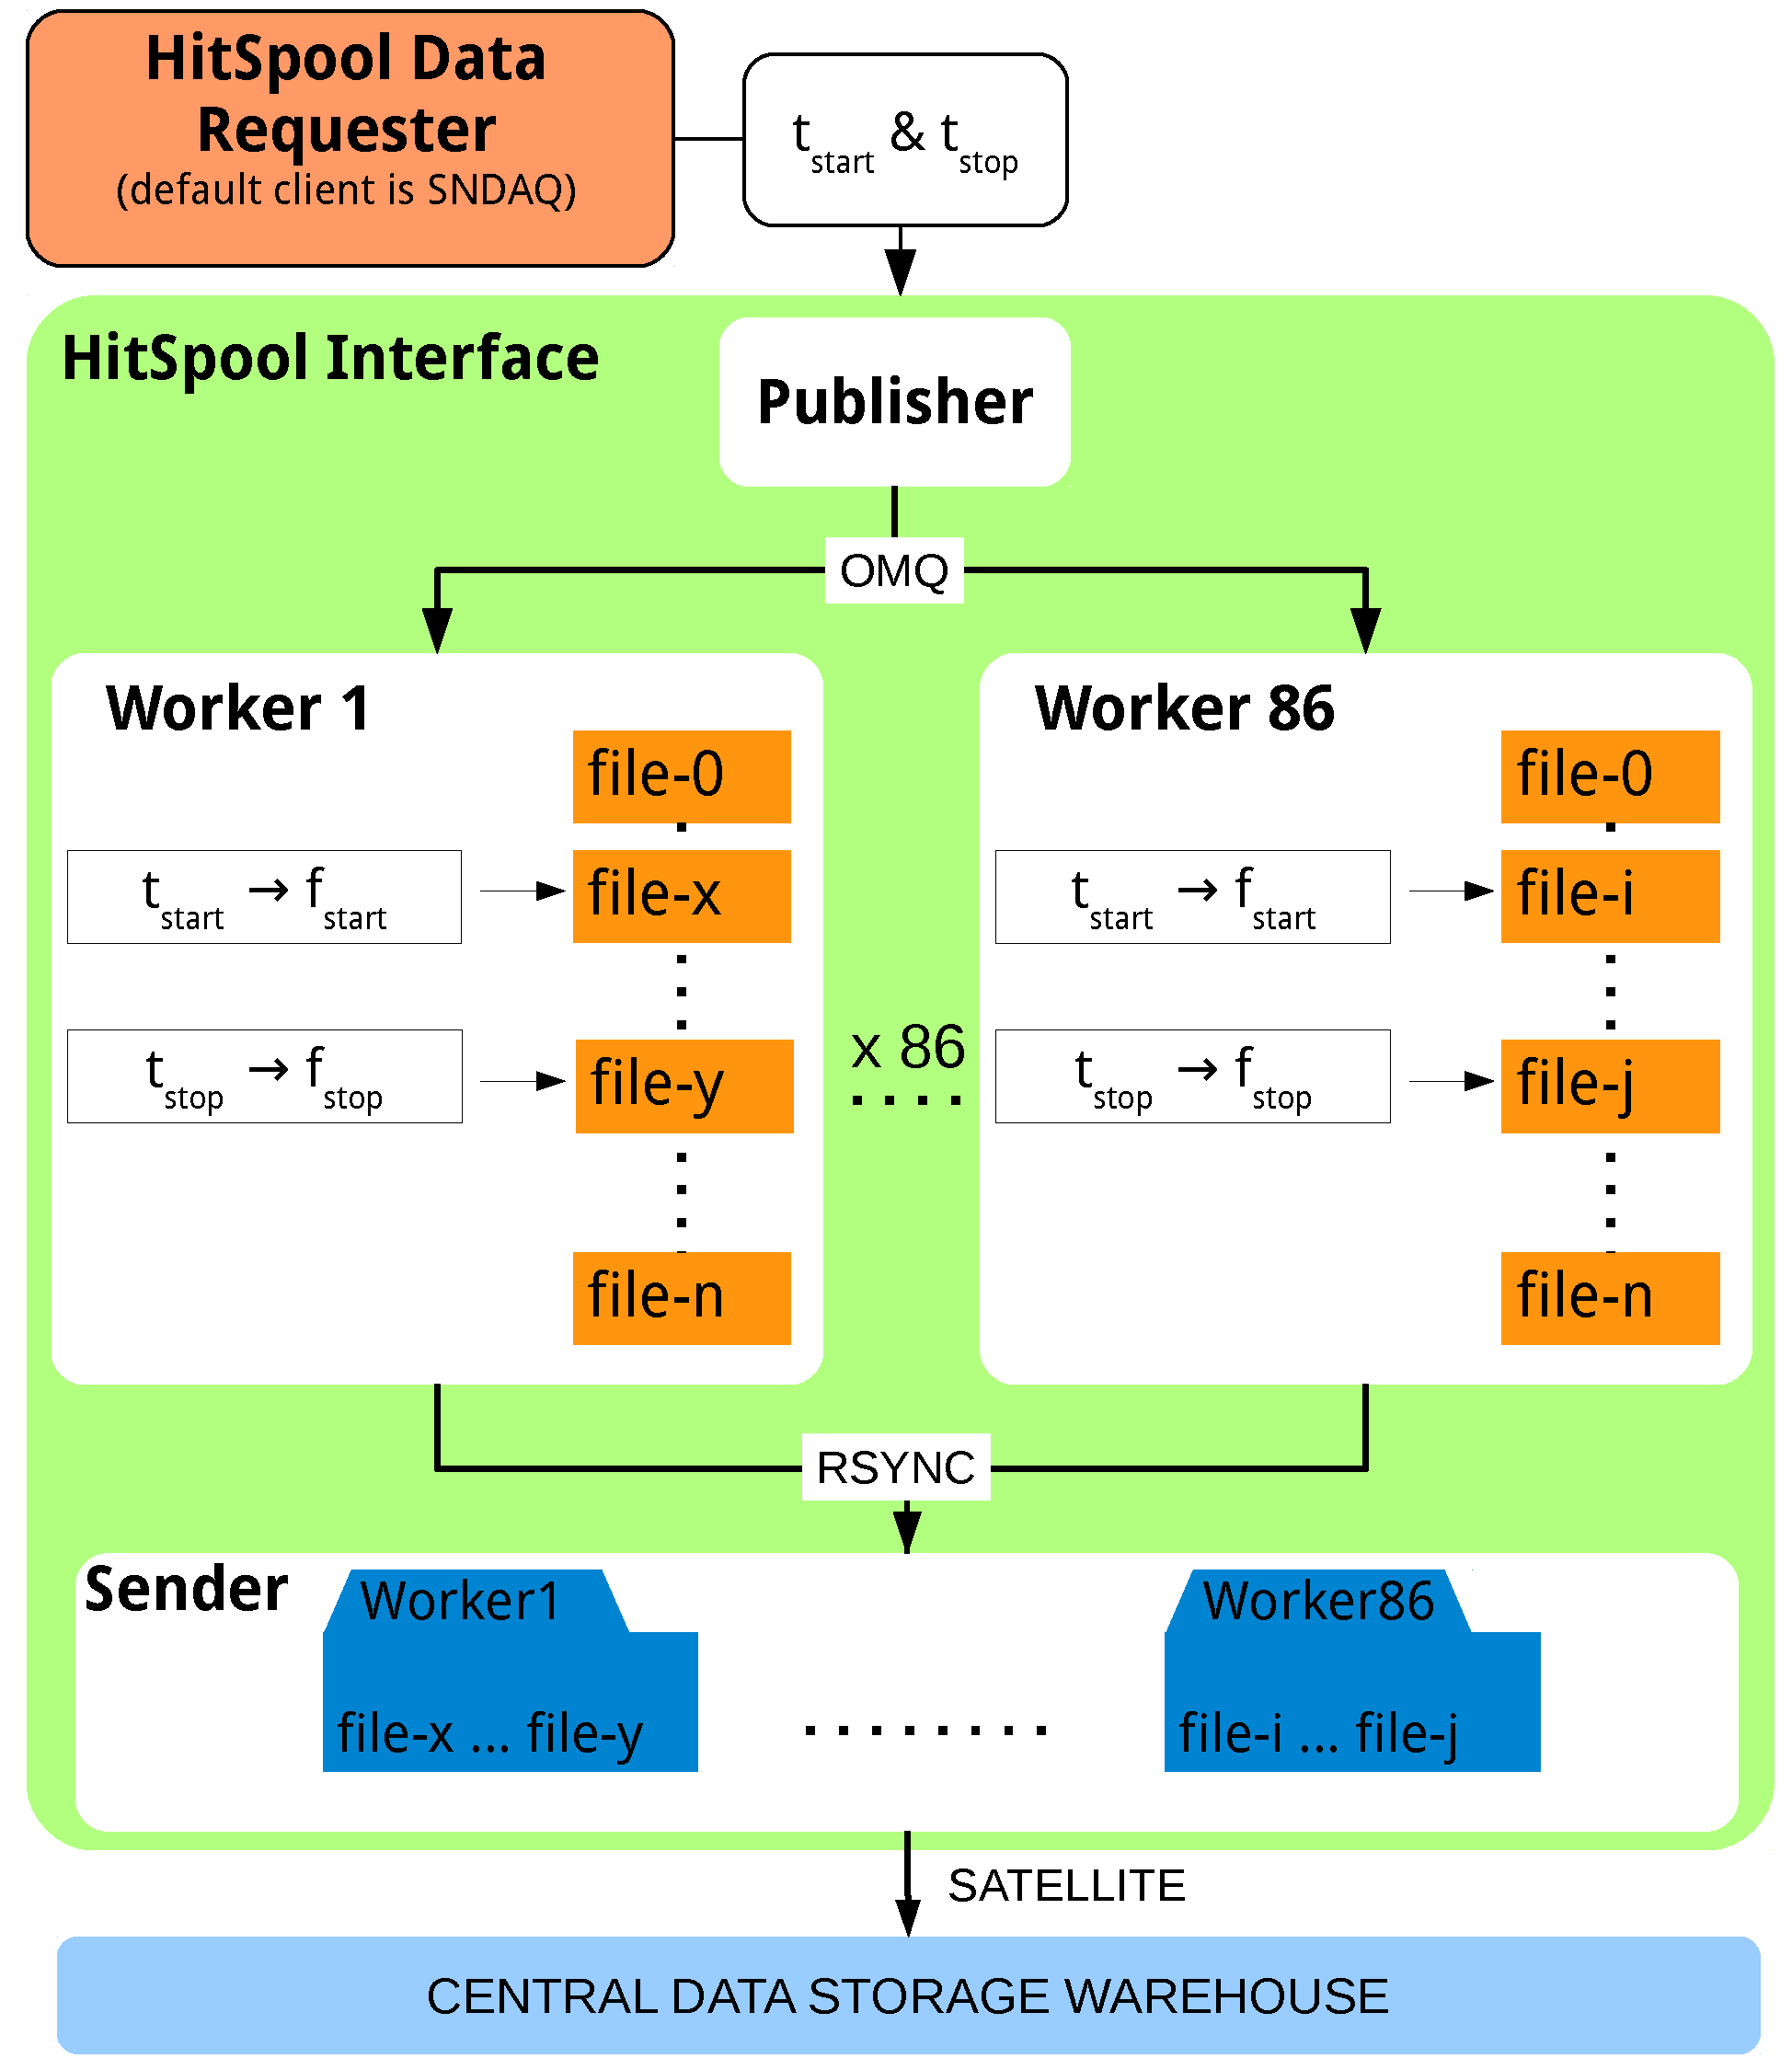
\includegraphics[width=\textwidth]{graphics/online/snstream/hsinterface_components_blockdiagram.pdf}
 \caption{Hitspool interface data flow}
 \label{fig:hsiface_dataflow}
 \end{minipage}
\hfill
 \begin{minipage}[t]{0.45\linewidth}
 \centering
  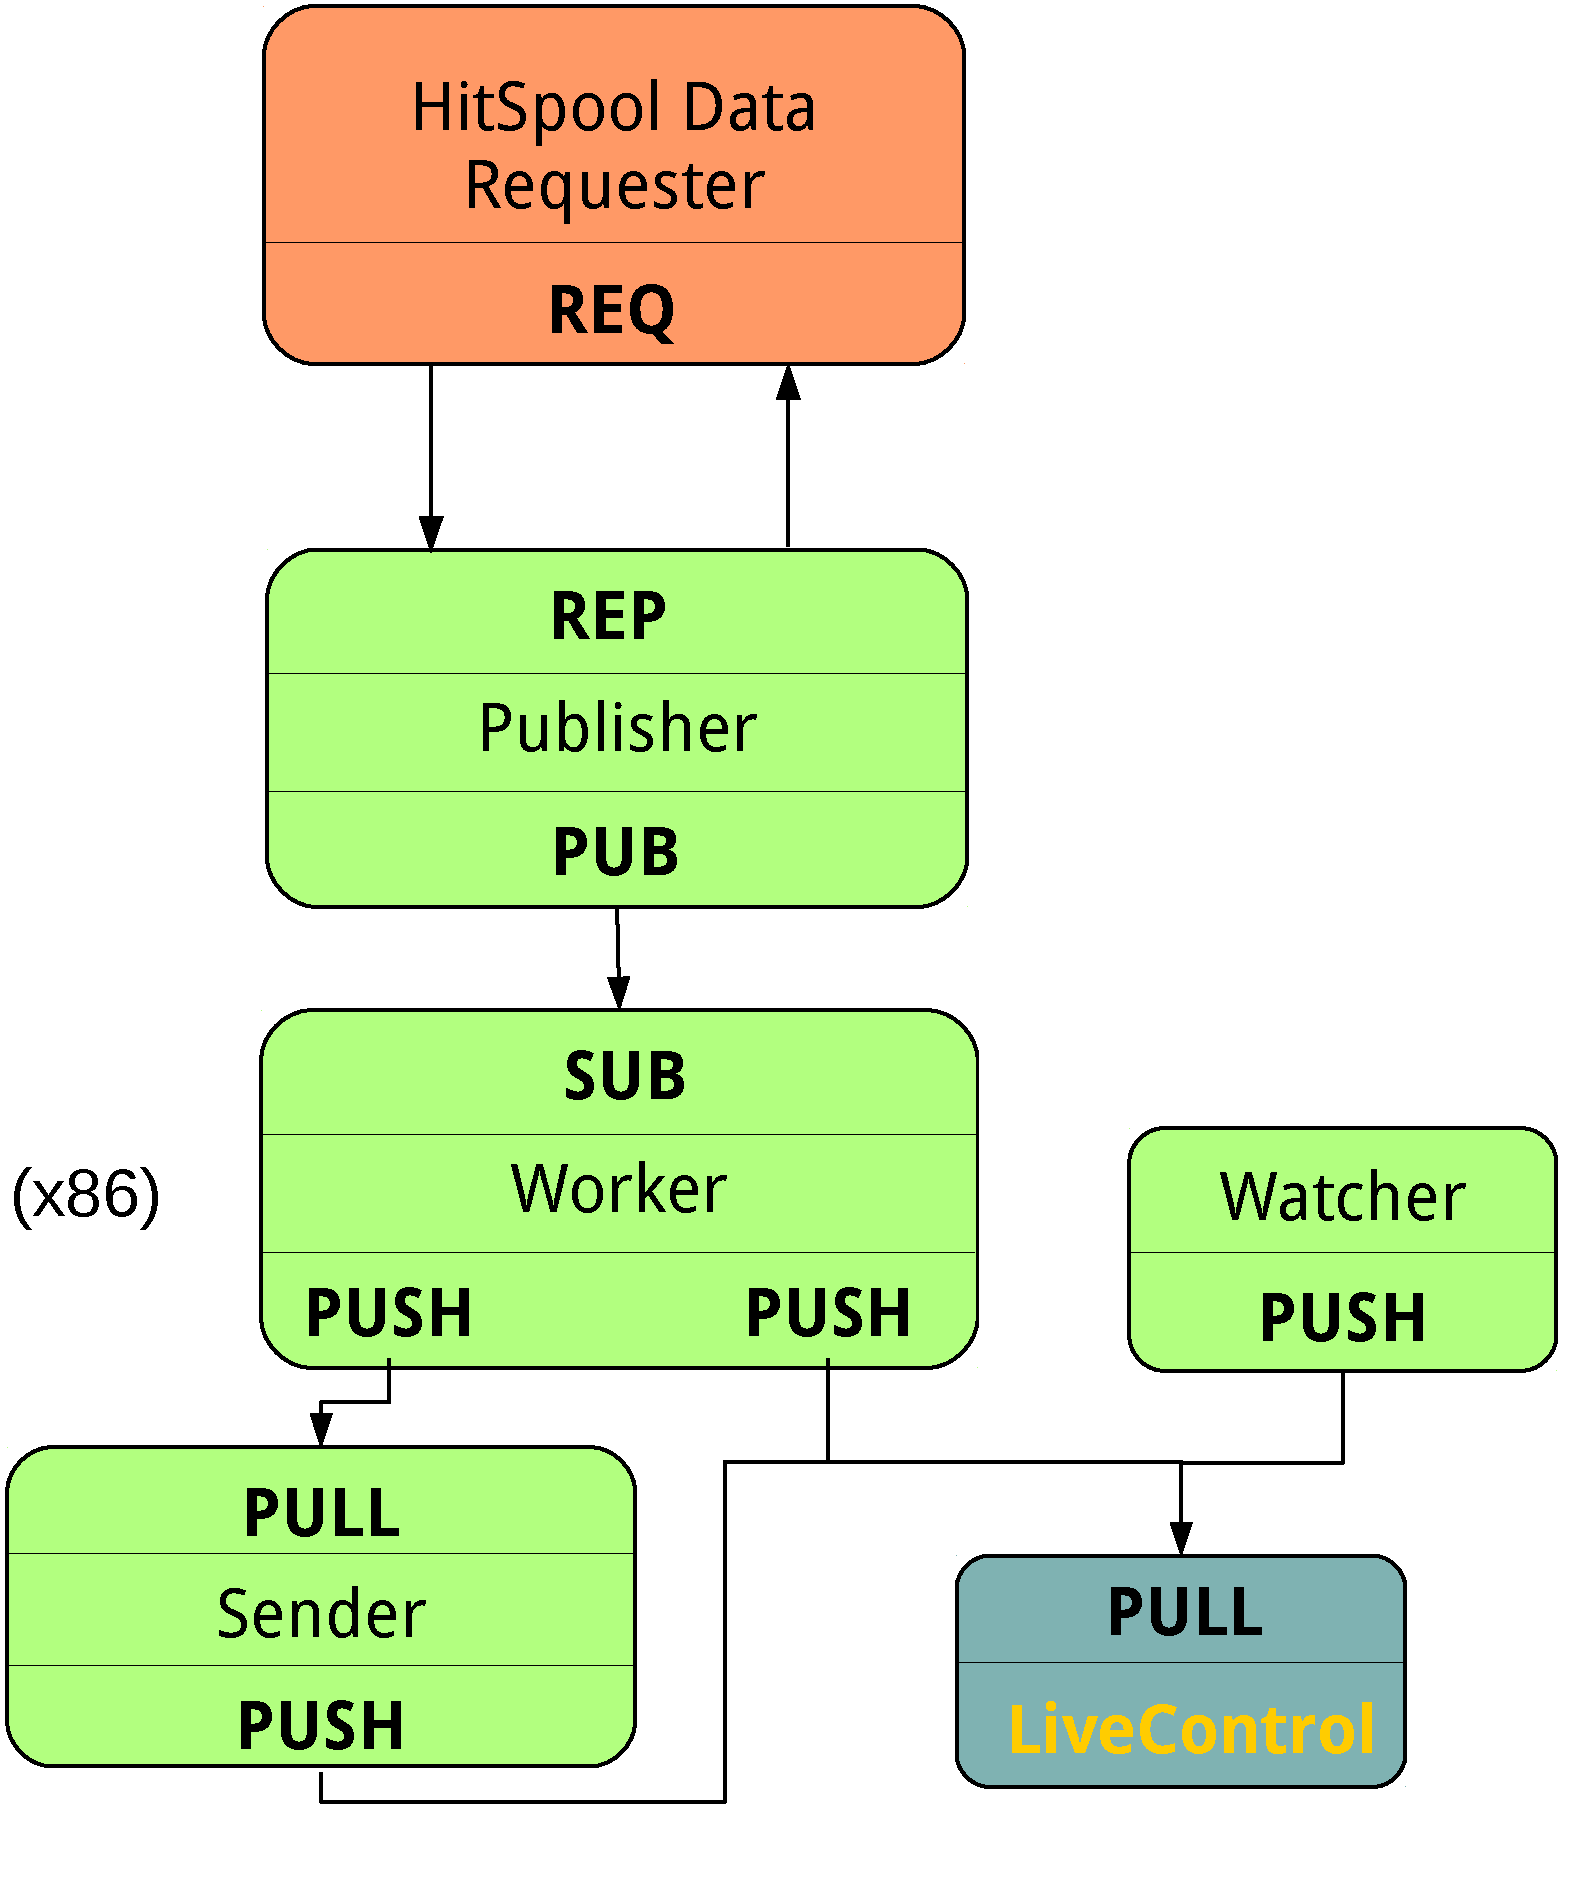
\includegraphics[width=\textwidth]{graphics/online/snstream/hsinterface_components_blockdiagram_msg_pattern.pdf}
 \caption{Hitspool interface messaging patterns}
 \label{fig:hsiface_msg_pattern}
 \end{minipage}
\end{figure}





\subsubsection{Triggers}

General description of trigger architecture.  Separation of trigger window
and readout window.  How trigger windows depend on geometry.  Thorough
escription of all different trigger algorithms. Trigger and readout window
merging. 

% Note: JK VLVnT proceedings may be useful here

Table: standard settings for triggers

Figure: trigger windows and readout windows.

Figure: example bright multi-trigger event.  

Figure: SLOP triplet geometry?

\subsubsection{Event Building}

Readout requests to StringHub components and packaging of waveforms into
events.  Spooling to disk and interface to PnF.

%\subsubsection{The Secondary Streams (SN/Moni/TCAL)}
%Is this necessary or can we just mention these in the StringHub section?

\subsubsection{Configuration}

Tree of XML configuration files for components, triggers, and DOM settings.  

\subsubsection{Distributed Network Control}

CnC server description.  XML-RPC.  

\subsection{Online Filtering}
\textsl{(Erik B.; 3-4 pages)}
\subsubsection{Overview}
Big picture view of what PnF is and does (route data from DAQ output to
files for pickup by data handling, applying calibration, recos and
filters along the way, TFT content, etc)

\subsubsection{System Design}
Cover the overall system design and tech used (CORBA, I3Inlet/I3Outlets,
etc) and how all pieces fit together and are controlled (mention
pf2live). Words about historical operation in Plan B in early seasons,
plan A.

\subsubsection{Components}
A brief description of each PnF component.
\paragraph{I3DAQDispatch}
\paragraph{PnF Server}
\paragraph{PnF Clients}
\paragraph{DB Cache}
\paragraph{Realtime Followup server and clients}

\subsubsection{Performance}
\paragraph{Overall rates and known limits (server + I/O limits)}
\paragraph{Average system latency}

Figure: plot of typical latency including run transition?

\subsection{Data Handling}
\textsl{(P. Meade; 1 page)}

Generation description of system architecture.  Stream definitions, dropboxes,
and data pickup.  Archival vs. transfer to TDRSS system.  

\subsection{I3Live and Remote Monitoring}
\textsl{(J. Braun; 1 page)}

I3Live duties of experiment control and realtime monitoring.  Component
descriptions.  Failover modes, alarms, and interface to paging system.
Monitoring system and Moni2.0.  Interface to ITS and its replacement
system, I3MS. 

\subsection{Operational Performance}
\textsl{(John K.; 1 page)}

Explanation of how design choices, system monitoring, and winterovers result in
high uptime.  Discussion of median downtime and various causes of downtime.
Possible basic failure analysis of hardware components.  

Figure: DAQ full uptime and clean uptime percentage.

Figure (optional): Downtime histogram.  
